\section{Knowing How with Linear Plans}
\label{sec:khlinearplans}

\subsection{Basic Definitions}

We start by introducing the most basic notion of knowing how as defined in e.g.~\cite{Wang15lori,Wang16,Wang2016}. Formulas describing the abilities of an agent of achieving a certain goal, are interpreted over Labeled Transition Systems, which indicate what actions are available for execution at each state, and how they transform one state into another.

% \begin{definition}\label{def:lts}
%     Let $\PROP$ be a countable set of propositional symbols. 
%     A \emph{Labeled Transition System (LTS)}  is a tuple
%     $\model=\tup{\S,\ACT,\ra,\V}$ such that:
%     \begin{itemize}
%         \item $\S$ is a countably non-empty set of states, \raul{Directamente finito?}
%         \item $\ACT$ is a countable set of action symbols,
%         \item ${\ra} \subseteq \S \times \ACT \times \S$ is a transition relation (sometimes we denote by $\reach{a}$ the set $\set{(s,t) \mid (s,a,t){\in}{\ra}}$, for $a\in\ACT$).
%     \end{itemize}
% \end{definition}

In order to determine when an agent knows how to achieve a goal, we need to characterize those sequences of actions (or plans) that result appropriate for such a purpose. This is the notion of \emph{strongly executable} plans about, indicating that a plan is ``fail proof''. This notion, discussed already in~\cite{Wang15lori,Wang16,Wang2016} was inspired by conformant planning (see e.g.~\cite{Smith&Weld98,Bonet2010}).

\begin{definition}\label{def:plans}
    Let $\model=\tup{\S,\ACT,\ra,\V}$ be an LTS. 
    Elements of $\ACT^*$ are called \emph{plans} (with $\epsilon$ the empty plan).  Let $\plan\in\ACT^*$, $\size{\plan}$ denotes its length ($\size{\epsilon}:=0$).
    For  $0\leq i \leq \size{\plan}$, the plan $\plan_i$ denotes the initial segment of $\plan$ up to (and including) the $i^{th}$ position (with $\plan_0 := \epsilon$). The action $\plan[i]$ is the one appearing in $\plan$ at the $i^{th}$ position. We define $\reach{\plan}$ as the composition $\reach{\plan[1]} \comp \ldots \comp \reach{\plan[\size{\plan}]}$. 

    We say that a plan $\plan\in\ACT^*$ is \emph{strongly executable (SE)} at a state $s\in\S$ if and only if, for all $0\leq i \leq \size{\plan}-1$ and all $t\in\S$ such that $s\reach{\plan_i} t$, there is $v\in\S$ such that $t\reach{\plan[i+1]} v$. The plan $\plan$ is SE at $T\subseteq \S$ if and only if it is SE at every $s\in T$. The notation $T \reach{\plan} U$ (for $T,U\subseteq\S$) indicates that for all $s\in T$, there is $t\in U$ such that $s\reach{\plan} t$.
\end{definition}

Now we are ready to introduce the language of knowing how.

\begin{definition}
    \label{def:syntax}
    The set of formulas (a.k.a. the language) of $\Khlogic$ is defined by the following BNF:
    \[
        \varphi, \psi ::= p \mid \neg \varphi \mid \varphi \vee \psi \mid \kh(\psi,\varphi),
    \]
    where $p\in\PROP$. Other Boolean operators are defined as usual. Formulas of the form $\kh(\psi,\varphi)$ are read as \emph{``the agent knows how to achieve $\varphi$ given $\psi$''}
\end{definition}

Formulas are interpreted over pointed LTS, i.e., w.r.t. an LTS and a given state. 

\begin{definition} \label{def:semantics-kh}
    Let $\model = \tup{\S,\ACT,\ra,\V}$ be an LTS and let $s\in\S$, the satisfiability relation $\models$ for $\Khlogic$ is inductively defined as:
    \[
    \begin{array}{l@{\ \ \ }c@{\ \ \  }l}
    \model, s \models p & \iffdef & p \in \V(s) \\
    \model, s\models \neg\varphi & \iffdef & \model, s \not\models \varphi \\
    \model, s \models \psi\vee\varphi & \iffdef & \model, s \models \psi \mbox{ or }\model, w \models \varphi \\
    \model, s \models \kh(\psi,\varphi) & \iffdef & \text{there is } \plan \in \ACT^* \;\text{such that:} \\
    & & \ \ \text{\rm (1)} \ \plan \text{ is SE at }  \truthset{\model}{\psi}\; \text{and} \\
    & & \ \ \text{\em (2)} \ \truthset{\model}{\psi} \reach{\plan} \truthset{\model}{\varphi}, 
    \end{array}
    \]      where: $\truthset{\model}{\chi} := \csetsc{s\in\S}{\model,w\models\chi}$. Define: $\model\models\varphi$ iff  $\truthset{\model}{\varphi}=\S$, and $\models\varphi$ iff $\model\models\varphi$, for all LTS $\model$.
\end{definition}

The model-checking problem for a given logic is defined as follows, where models and formulas are instantiated with those corrresponding to each particular case. 

\begin{description} \itemsep 0cm
    \item[Input:] A model $\model$, a state $s$ in $\model$ and a formula $\varphi$;
    \item[Output:] $\model,s\models\varphi$?
\end{description}

\begin{proposition}[\cite{DemriF23}]
    The model-checking problem for $\Khlogic$ is \PSPACE-complete.
\end{proposition}

\subsection{The Probabilistic Approach}

Naturally, our first approach will be extending $\Khlogic$ with some form of probabilistic behaviour. 

% We will start by introducing PLTS, an extension of LTS with probabilities.

% \begin{definition}\label{def:plts}
%     Let $\PROP$ be a countable set of propositional symbols. 
%     A \emph{Probabilistic Labeled Transition System (PLTS)}  is a tuple
%     $\model=\tup{\S,\ACT,\ra,\V}$, defined exactly as an LTS except that ${\ra}\subseteq \S \times \ACT \times \dist(\S)$, where  $\dist(\S)$ is the set of probability distributions over $\S$.
% \end{definition}

% We will start by introducing PLTS, an extension of LTS with probabilities.

% \begin{definition}\label{def:plts}
%     Let $\PROP$ be a countable set of propositional symbols. 
%     A \emph{Probabilistic Labeled Transition System (PLTS)}  is a tuple
%     $\model=\tup{\S,\ACT,\ra,\V}$, defined exactly as an LTS except that ${\ra}\subseteq \S \times \ACT \times \dist(\S)$, where  $\dist(\S)$ is the set of probability distributions over $\S$.
% \end{definition}

\begin{figure}[t]
    \begin{center}
        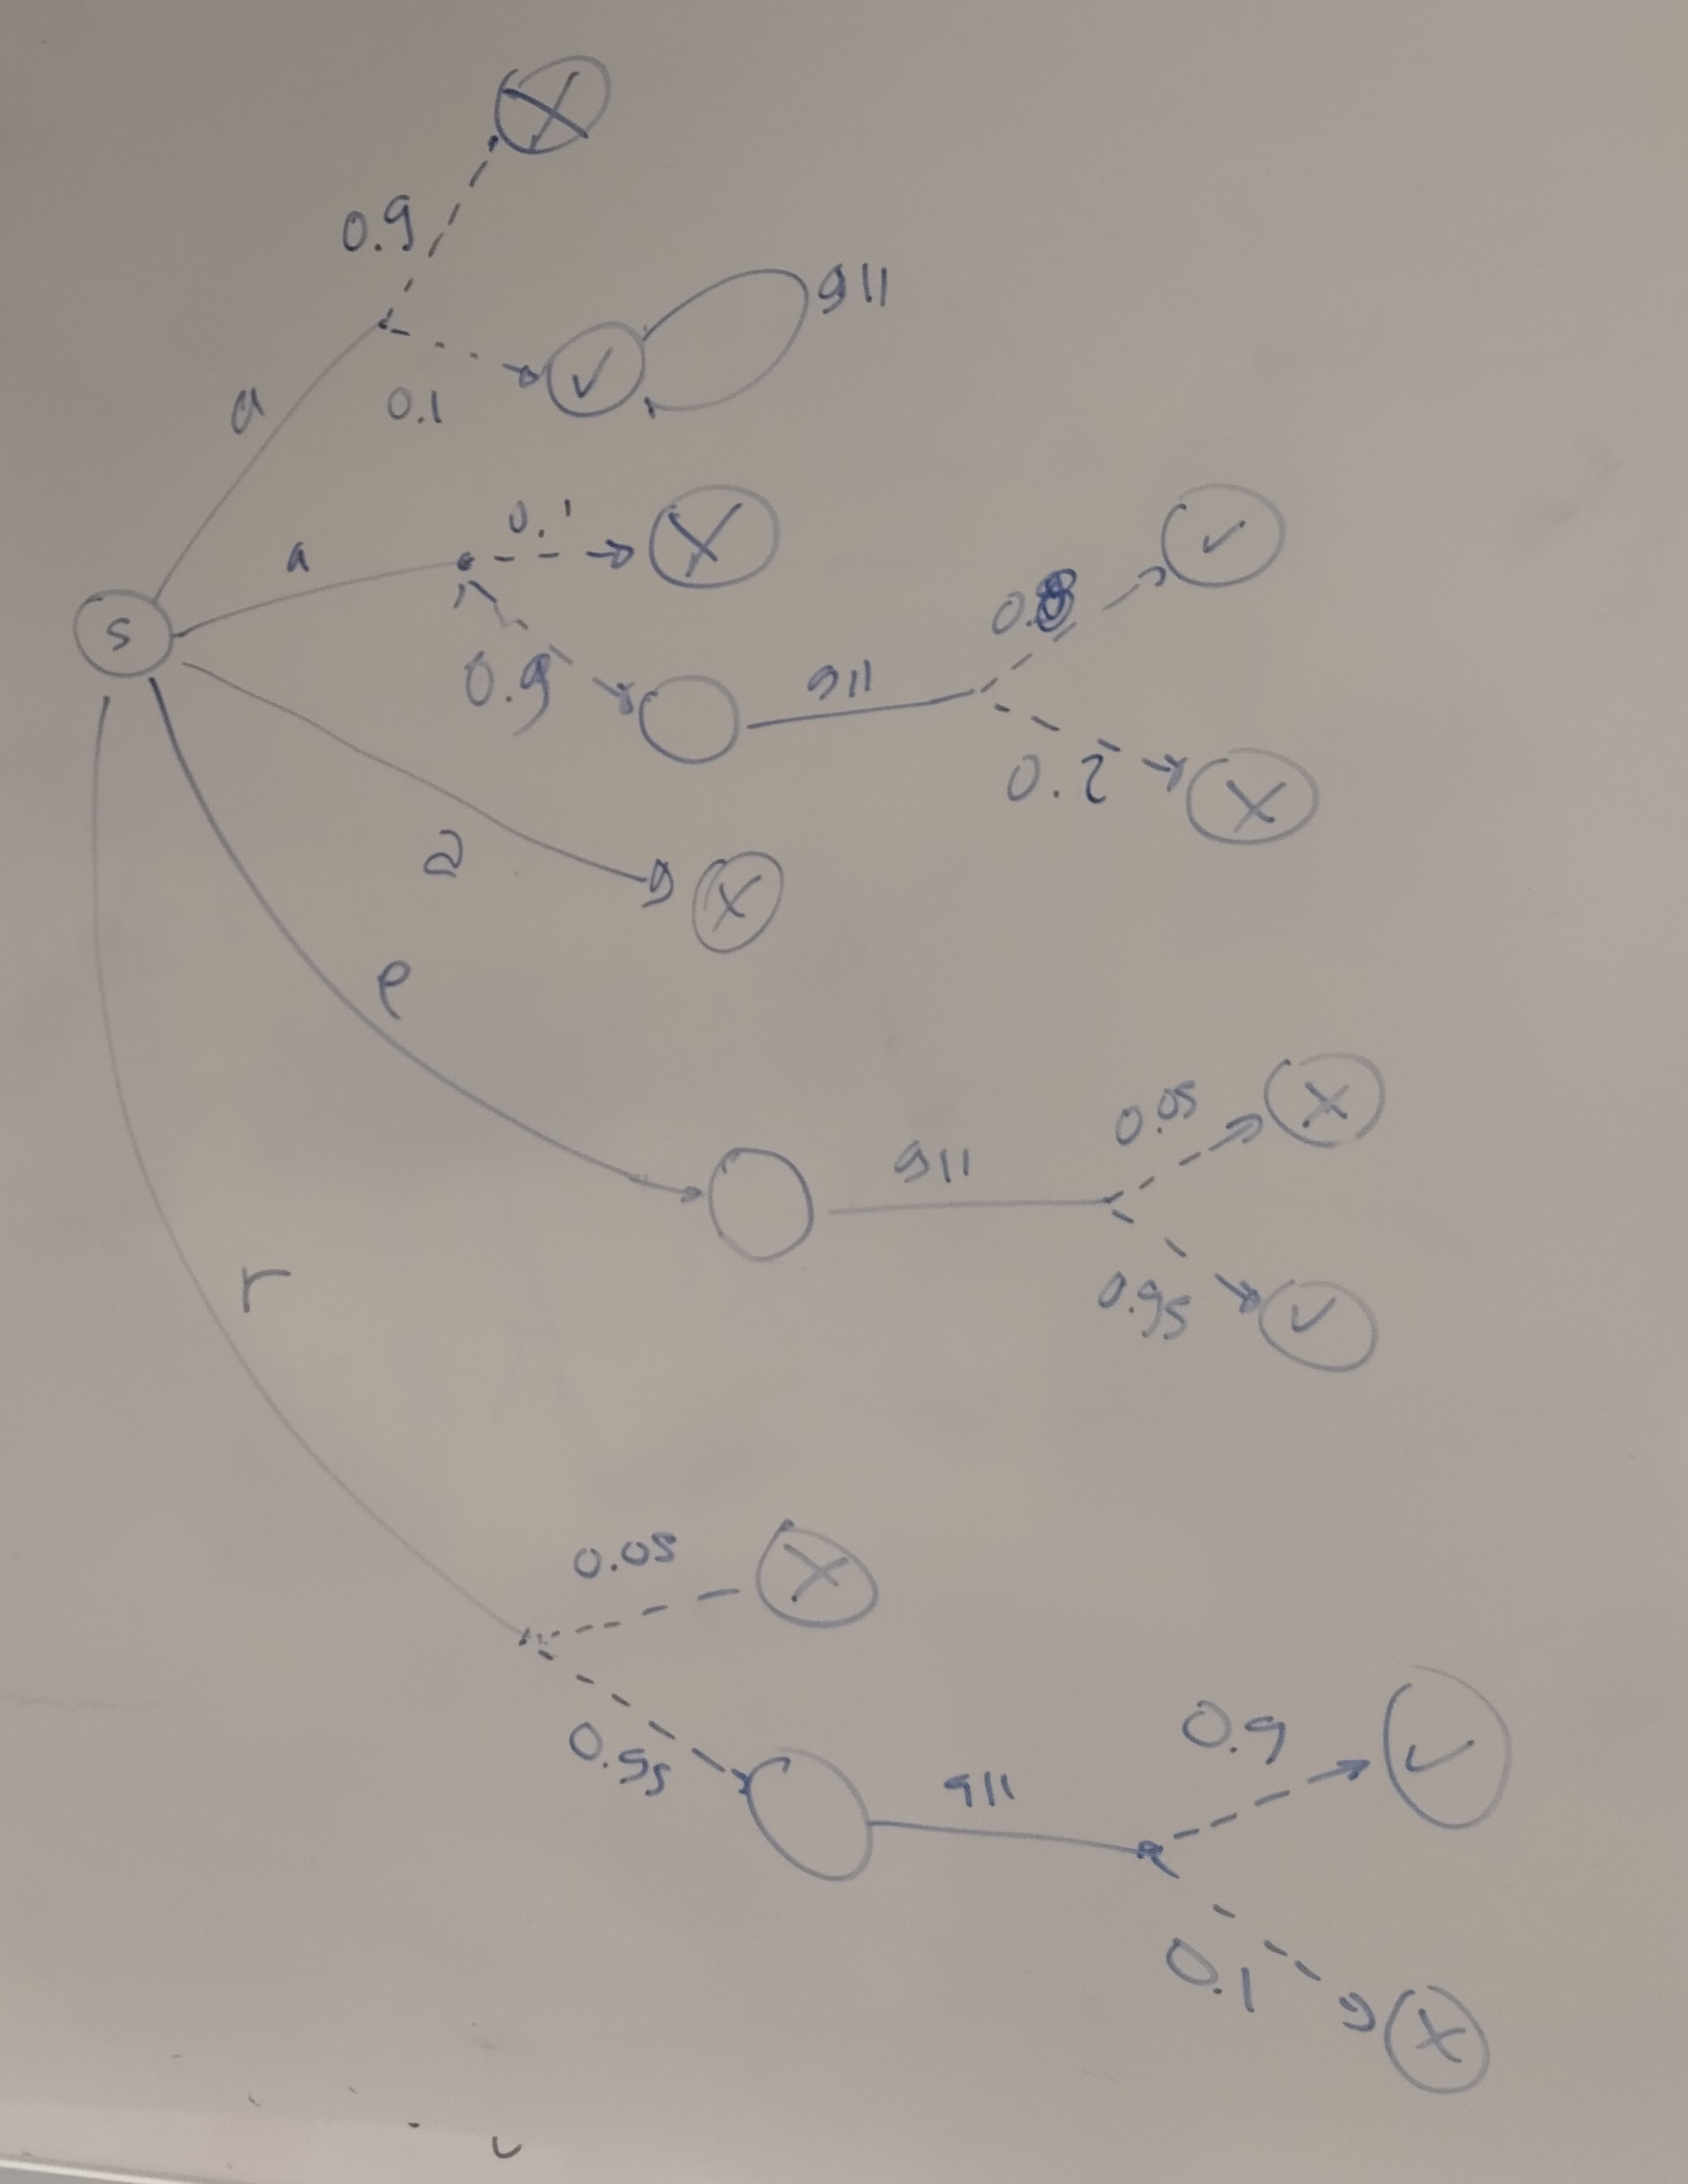
\includegraphics[scale=0.1]{PLTS.jpg}
    \end{center}
\end{figure}

% We need to capture the notion of executability with probability at least $q$, for some $q\in[0,1]$. 

% \begin{definition}\label{def:strategy-comp-exec}
%     Let $\model=\tup{\S,\ACT,\ra,\V}$ be a PLTS, a \emph{strategy} is a function $\strat: \S\times(\ACT\times\S)^* \ra \dist(\S\times\ACT\times\dist(\S))$. Let $\plan\in\ACT^*$, we say that $\strat$ is \emph{$\plans$-compatible} if and only if, for all $\rho\in \S\times(\ACT\times\S)^*$, the following conditions hold:
%     \begin{enumerate}
%         \item $\strat(\rho)(s,a,\mu)>0$ implies $\last(\rho)=s$ and $s\reach{a}\mu$ in $\model$, and 
%         \item $\bar{\rho}\in\pref(\plans)$ implies $\bar{\rho}a\in\pref(\plans)$.
%     \end{enumerate}
%     For $\plan\in\ACT^*$, we say that $\sigma$ is \emph{$\plan$-compatible} if it is $\{\plan\}$-compatible. 

%     Let $q\in[0,1]$, we say that $\plans$ is \emph{$q$-executable} at $s\in\S$, if and only if, 
%     \[
%         \infim_{\{\strat \mid \strat \text{ is } \plans\text{-comp.}\}} \Prob^\strat_{s}(\plans)\geq q.
%     \]
%     Finally, $\plans$ is \emph{$q$-executable} at $B\subseteq\S$, if and only if, it is $q$-executable at every $s\in B$. 
%     A plan $\plan$ is \emph{$q$-executable} at $s$ (respectively, at $B$) if $\{\plan\}$ is $q$-executable at $s$ (respectively, at $B$). 
% \end{definition}

% \bigpedro{todo lo de arriba en esta subsecci\'on deber\'ia irse, la mayor\'ia de las cosas est\'an definidas en los preliminaries, queda la idea de $\plans$-compatible que viene debajo}



Given a set of plans $\plans\subseteq\ACT^*$, we want to consider
strategies that follow as faithfully as possible the plans of
$\plans$.  Therefore, we say that a strategy $\sigma$ is
\emph{$\plans$-compatible} if for all $\rho\in\execf$ such that
$\bar{\rho}\in\pref(\plans)$,
%
\begin{enumerate}
\item%
  $\strat(\rho)(a,\mu)>0$ implies $\bar{\rho}a\in\pref(\plans)$, and
\item%
  $\strat(\rho)(\complete)>0$ implies that either
  $\bar{\rho}\in\plans$ or
  $\bar{\rho}\{a\mid{\last(\rho)\reach{a}\mu}\}\cap\pref(\plans) = \emptyset$. 
\end{enumerate}
%
The first item states that $\strat$ can chose an $a$-labelled
transition after the partial plan $\bar{\rho}$ if the continuation of
$\bar{\rho}a$ is also a partial plan.
%
The second item states that $\strat$ is allowed to terminate after the
partial plan $\bar{\rho}$ if either $\bar{\rho}$ is itself a valid
plan, or $\bar{\rho}$ cannot be continued by the PLTS within some
valid plan.
%
Let $\Comp(\plans)$ denote the set of all $\plans$-compatible
strategies.
%
%% Given a plan $\plan\in\ACT^*$, we say that a strategy $\strat$ is
%% $\plan$-compatible iff it is $\{\plan\}$-compatible.
\pedro{poner ejemplos de $\plans$-compatible respecto de alg\'un running
  example}


Let $\plans$ be a set of plans that are believed to perform
equivalently in order to reach some goal state in $G\subseteq\S$.  We
define the set of \emph{successful complete (finite) execution} that
reach $G$ following some plan in $\plans$ by
$\Succ(\plans,G)=\{{\rho\complete\in\cexecf}\mid{\bar{\rho}\in\plans
  \text{ and } \last(\rho)\in G}\}$.
%
We are interested in that any $\plans$-compatible strategy $\sigma$
starting from a given state $s\in\S$ reaches a state in $G$ with a
minimum desired probability, say $q$.  That is, we would like that
%
\begin{equation}\label{eq:plans:goal:q}
  \inf_{\sigma \in\Comp(\plans)}\Prob^\strat_s(\Succ(\plans,G)) \geq q.
\end{equation}
%
More generally, we would like that this holds from any particularly
assumed state in a set $A\subseteq\S$ (say, a precondition).  So, we
write $A \reach{\plans}_q G$ if and only if for all state $s\in A$,
the condition in \cref{eq:plans:goal:q} holds.
%
Thus $A \reach{\plans}_q G$ means that any state in $A$ can reach the
goal $G$ with at least probability $q$ following some plan in $\plans$
\textcolor{red}{in an adaptively manner}.
\pedro{ejemplo de esto tambi\'en}


\bigpedro{creo que es importante pensar ahora la estructura del paper}




\bigpedro{desde el cartel hasta aqu\'i es nuevo}



Notice that, whenever $q=1$, we are in the case of SE from~\Cref{def:plans}. \raul{Chequear esto} The extended language with probabilities is given below.


\begin{definition}
    \label{def:syntax-extended}
    The set of formulas (a.k.a. the language) of $\Khlogic$ is defined by the following BNF:
    \[
        \varphi, \psi ::= p \mid \neg \varphi \mid \varphi \vee \psi \mid \kh^q(\psi,\varphi),
    \]
    where $p\in\PROP$ and $q\in[0,1]$. Other Boolean operators are defined as usual. Formulas of the form $\kh(\psi,\varphi)$ are read as \emph{``the agent knows how to achieve $\varphi$ given $\psi$ with probability at least $q$''}.
\end{definition}




Now we proceed by introducing the semantics of the new modality.

\begin{definition}
    Let $\model = \tup{\S,\ACT,\ra,\V}$ be a PLTS and let $s\in\S$, the satisfiability relation $\models$ for $\PKh$ is inductively defined as:
    \[
        \begin{array}{l@{\ \ \ }c@{\ \ \  }l}
        % \model, s \models p & \iffdef & p \in \V(s) \\
        % \model, s\models \neg\varphi & \iffdef & \model, s \not\models \varphi \\
        % \model, s \models \psi\vee\varphi & \iffdef & \model, s \models \psi \mbox{ or }\model, w \models \varphi \\
        \model, s \models \kh^q(\psi,\varphi) & \iffdef & \text{there is } \plan \in \ACT^* \;\text{such that:} \\
        & & \ \ \text{\rm (1)} \ \plan \text{ is $q$-executable at }  \truthset{\model}{\psi}\; \text{and} \\
        & & \ \ \text{\em (2)} \ \truthset{\model}{\psi} \reach{\plan}_q \truthset{\model}{\varphi}, 
        \end{array}
        \] \raul{1 and 2 will be merged into one condition.}
        where: $\truthset{\model}{\chi} := \csetsc{s\in\S}{\model,w\models\chi}$. Define: $\model\models\varphi$ iff  $\truthset{\model}{\varphi}=\S$, and $\models\varphi$ iff $\model\models\varphi$, for all PLTS $\model$.
\end{definition}

\begin{theorem}\label{th:mc-khp-undecidable}
The model-checking problem for $\PKh$ is undecidable.
\end{theorem}

\begin{proof}
    Suppose we want to check whether $\model,s\models\kh^q(\psi,\varphi)$.  W.l.o.g., consider $\model$ is complete and deterministic. 
    From the semantics, we need to check if there is $\plan\in\ACT^*$ satisfying conditions (1) and (2). Consider condition (1), i.e., we need to check whether $\plan$ is $q$-executable at all $s\in\truthset{\model}{\psi}$. Fix such an $s$. Since $\model$ is deterministic and complete, it all boils down to check whether there is $\plan\in\ACT^*$ such that $\Prob^\strat_s(\plan)\geq q$ (notice that $\strat$ is unique by determinism of $\model$). 
    The latter solves the problem of checking whether the language recognized by a probabilistic (deterministic) automata is empty, which is undecidable~\cite{MadaniHC99}. 
\end{proof}

\subsection{Indistinguishability Classes in Knowing How}
